\documentclass[10pt,twocolumn,letterpaper]{article}

\usepackage{iccv}
\usepackage{times}
\usepackage{epsfig}
\usepackage{graphicx}
\usepackage{amsmath}
\usepackage{amssymb}

% Include other packages here, before hyperref.

% If you comment hyperref and then uncomment it, you should delete
% egpaper.aux before re-running latex.  (Or just hit 'q' on the first latex
% run, let it finish, and you should be clear).
\usepackage[breaklinks=true,bookmarks=false]{hyperref}

\iccvfinalcopy % *** Uncomment this line for the final submission

\def\iccvPaperID{****} % *** Enter the ICCV Paper ID here
\def\httilde{\mbox{\tt\raisebox{-.5ex}{\symbol{126}}}}

% Pages are numbered in submission mode, and unnumbered in camera-ready
\ificcvfinal\pagestyle{empty}\fi

\begin{document}

%%%%%%%%% TITLE
\title{Self-Distillation using image-language representation for image classification}

\author{Pasit Tiwawongrut\\
Asian Institute of Technology\\
Klong Luang Pathumthani 12120, Thailand\\
{\tt\small Pasit.Tiwawongrut@ait.asia}
% For a paper whose authors are all at the same institution,
% omit the following lines up until the closing ``}''.
% Additional authors and addresses can be added with ``\and'',
% just like the second author.
% To save space, use either the email address or home page, not both
\and
Dr. Chaklam Silpasuwanchai\\
Asian Institute of Technology\\
Klong Luang Pathumthani 12120, Thailand\\
{\tt\small chaklam@ait.asia}
}

\maketitle
% Remove page # from the first page of camera-ready.
\ificcvfinal\thispagestyle{empty}\fi

%%%%%%%%% ABSTRACT
\begin{abstract}
   The ABSTRACT is to be in fully-justified italicized text, at the top
   of the left-hand column, below the author and affiliation
   information. Use the word ``Abstract'' as the title, in 12-point
   Times, boldface type, centered relative to the column, initially
   capitalized. The abstract is to be in 10-point, single-spaced type.
   Leave two blank lines after the Abstract, then begin the main text.
   Look at previous ICCV abstracts to get a feel for style and length.
\end{abstract}

%%%%%%%%% BODY TEXT
\section{Introduction}

Vision language pre-trained models have shown effective performance in both in-domain and downstream tasks by utilizing both text and image information.
CLIP \cite{clip} and ALIGN \cite{align} train image and text encoders with contrastive learning to align vision and language modalities, which results in competitive performance in many vision language tasks \eg image-text retrieval, visual question answer, and zero-shot image classification.
ALBEF \cite{albef}, CoCa \cite{coca} and mPLUG \cite{mplug} added cross-attention layers over image and text encoders to provide better alignment over vision and language modalities with multiple training objectives \eg image-text captioning, image-text contrastive loss, image-text matching and masked-language-modeling loss.
As a result these models achieved state-of-the-art multiple vision-language and image classification task.

However, the gap in using the self-distillation to improve vision language model performance for downstream task was still underexplored. 
By using the moving average teacher \cite{mean_teacher,eman}, the teacher model weight is updated with the average of the student model gradient. 
As a result, the teacher model output representation is consistent.
MixMatch \cite{mixmatch}, Mixup \cite{mixup}, and Fixmatch \cite{fixmatch} are image input interpolation methods for improving output consistency within the teacher-student framework by image augmentation and input interpolation between each sample.
Our work is inspired by DINO \cite{dino} which utilizes both moving average teacher and image interpolation techniques to train the teacher-student image encoder model without using any label, which results in competitive down-stream task performance.

In this paper, we proposed a method to improve the performance of the image and text encoder vision language model using the self-distillation \cite{mean_teacher} technique as shown in Figure \ref{fig:overall_method}.
LiT \cite{lit} showed that with the image and text encoders architecture, the freezing image encoder and tuning only the text encoder for the downstream tasks can perform better than tuning both image and text encoders.
By using the moving average teacher, we can remove noise from the text encoder model, which is trained using noisy internet image-text pairs.
In order to produce a robust text encoder, interpolated text input is required for moving average teacher methods.
%% TODO: clarify why I choose two-stream pre-trained model.
We provided the result by applying our method over pre-trained vision language models in image classification and cross-modal retrieval tasks compared to the finetuning method.
%% TODO: Identify finetuning method.
The main contribution of our work was to utilize the moving average teacher to improve downstream task performance for the pre-trained vision language model.

\begin{figure}[h]
   \label{fig:overall_method}
   \begin{center}
      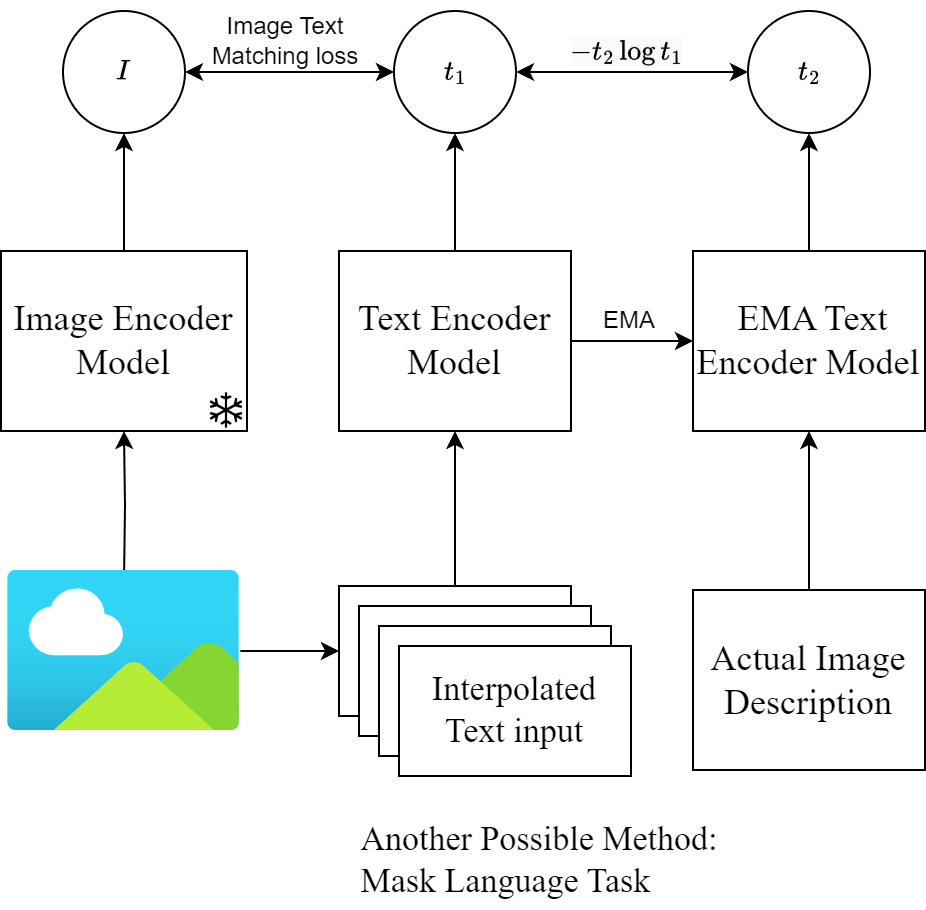
\includegraphics[width=0.8\linewidth]{Images/ThesisDiagram.png}
   \end{center}
   \caption{Overview of proposed method of applying moving average teacher to produce robust text encoder in pre-trained vision language model.}
   \small
\end{figure}


\section{Related work}

\subsection{Vision-Language model}
In the past few years, many works have shown the ability to utilize textual information with the image task by training with image text pair \eg CLIP \cite{clip}, UNITER \cite{uniter}, Blip \cite{blip-1,blip-2}, BEiT \cite{beit-3} and CoCa \cite{coca}.
By training with a large amount of the image-text pair dataset, the ALIGN model could make up for the noisy image description and surpass the model, which was trained with the benchmark dataset in the zero shot image classification task.
Recently \textbf{Co}ntrastive \textbf{Ca}ptioner (CoCa) \cite{coca} proposed a vision-language encoder-decoder model which was trained with image-text contrastive loss and captioning loss
Cross attention layers were added to join image-text modality.
The CoCa model performed linear probing image classification on ImageNet with top-1\% 90.6\% accuracy.
In this research, we adopted the two stream encoder method same as CLIP, and we also used a cross attention layer to create image-text representation for classification.
Another methods \cite{uniter,beit-3,uniter,vlmo} is to concatenate both image and text embedding and utilize multi-head self-attention to joined vision and language modalities.

\subsection{Knowledge Distillation and Self-Distillation}
Knowledge Distillation was firstly proposed by \cite{knowledge_distill} to compress the model size while maintaining the model performance as much as possible.
The method contained a smaller student model and a single or multiple larger teacher model.
The knowledge was transferred by optimizing the student model output to match the teacher's output.
\cite{born_again} investigated knowledge distillation using a student model size the same as the teacher model, showing improvement in the student model.
Such a method is called self-distillation.
The self-distillation has widely adopted in semi-supervised image classification tasks, such as Mean Teacher \cite{mean_teacher}, EMAN \cite{eman} and FixMatch \cite{fixmatch}.
DINO \cite{dino} proposed self-distillation pre-training without using any label, which resulted in performance improvement.
In this paper, we extended the self-distillation by creating representation which was image-text combined representation, and we trained the student model to match teacher softmax outputs.

\section{Methodology}
In this section we provided our self-distillation method and experiment setup details.
\subsection{Self-Distillation}
   
\subsection{Evaluation}


{\small
\bibliographystyle{ieee_fullname}
\bibliography{references}
}

\end{document}
